\title{CSCI 6150, Project Report}
\author{
        Caleb Adams \\
                Department of Computer Science\\
}
\date{\today}

% https://oeis.org/wiki/List_of_LaTeX_mathematical_symbols

\documentclass[12pt]{article}

\usepackage{graphicx}
\usepackage{subcaption}
\usepackage{tikz}
\usepackage[margin=1.5cm]{geometry}
\usepackage[most]{tcolorbox}
\usepackage{chessboard}
\usepackage{float}
\usepackage{hyperref}
%\usepackage{fontspec}
\usepackage{siunitx}
\usepackage{amsfonts}
\usepackage{amsmath}
\usepackage{amssymb}

\newcommand*\circled[1]{\tikz[baseline=(char.base)]{
            \node[shape=circle,draw,inner sep=2pt] (char) {#1};}}

\storechessboardstyle{4x4}{maxfield=d4}
\usetikzlibrary{arrows,automata}

\newtcblisting{commandshell}{colback=black,colupper=white,colframe=black!75!black,
listing only,listing options={language=sh},
every listing line={\textcolor{green}{\small\ttfamily\bfseries Caleb Adams \$> }}}

\begin{document}
\maketitle

\section{Introduction}

The goal of this project is to use material learned in the CSCI 6150 class to simulate
a Cart Pole system. The most heavily referenced materials for this project were the
Underactuated Robotics course materials from MIT \cite{underactuated} and the various
papers of Mattew Peter Kelly \cite{mattkelly}, though additional materials were used.

\begin{figure}[!ht]
 \centering
 \includegraphics[width=0.4\textwidth]{img/diagram1}
 \caption{A diagram of the Cart Pole system, which is a pendulum attached to a rolling cart.\cite{mattkelly}}
 \label{fig:oof}
\end{figure}

The Cart Pole system consists of a Cart, which is free to roll in the x directions, and a
pendulum which is free to rotate around the center of the cart. The pole and the cart
transfer energy between one another, with the total energy of the system being constant.
Only friction and damping due to wind resistance would remove energy from the system.
Once should also consider that the Cart and the Pole are exerting forces of varying magnitudes
on one another over time. This is was allows the system to be described as a set of
second order equations. A video of the simulation can be found at the link \url{https://youtu.be/kN71HXND6Nw}

\newpage

\section{Dynamics of the Cart Pole}

A Balance of forces can be see on the Cart Pole in Figure 2. This balance of forces
is what is used to generate the equations which govern the Cart Pole.

\begin{figure}[!ht]
    \centering
    \begin{subfigure}[b]{0.3\textwidth}
        \includegraphics[width=\textwidth]{img/diagram2}
        \caption{The freebody diagrams describing the Cart Pole.\cite{mattkelly}}
        \label{fig:asd123}
    \end{subfigure}
    ~ %add desired spacing between images, e. g. ~, \quad, \qquad, \hfill etc.
      %(or a blank line to force the subfigure onto a new line)
    \begin{subfigure}[b]{0.3\textwidth}
        \includegraphics[width=\textwidth]{img/diagram3}
        \caption{Diagram of the Symbols used for the Cart Pole system.}
        \label{fig:qwerty}
    \end{subfigure}
    \caption{Diagrams of the Cart Pole}\label{fig:asdfasdf}
\end{figure}

From these free body diagrams, we can generate 3 equations (the force balance on the cart,
the balance on the pole, and the balance around the pivot):

\begin{equation} \label{eq:1}
(F - T) \hat{i} + (N - W_1 - T_y) \hat{j} = m_1 \ddot{p_1}
\end{equation}

\begin{equation} \label{eq:2}
(T_x) \hat{i} (T_y - W_2 ) \hat{j} = m_2  \ddot{p_2}
\end{equation}

\begin{equation} \label{eq:3}
(T_x) \hat{i} (T_y - W_2 ) \hat{j} = m_2  \ddot{p_2}
\end{equation}

In the end, these equations give us the following second order linear system to
describe the cart pole \cite{mattkelly} \cite{underactuated}:

\begin{equation} \label{eq:4}
\begin{bmatrix}
\cos \theta & l \\
m_1 + m_2 & m_2 l \cos \theta
\end{bmatrix}
\begin{bmatrix}
\ddot{x} \\
\ddot{\theta}
\end{bmatrix}
=
\begin{bmatrix}
- g \sin \theta \\
F + m_2 l \dot{\theta}^2 \sin \theta
\end{bmatrix}
\end{equation}

For the purpose of this project I transform this system back into two functions.
This system can be viewed as $A x = b$, so simply $x = A^{-1} b$ will give us
a solution. Then, we can solve for the second derivatives. Doing this yields the following
two equations:

\begin{equation} \label{eq:5}
\ddot{x} = \frac{-g \sin \theta m_2 l \cos \theta + (-l)(F + m_2 l \dot{\theta}^2 \sin \theta) }{ (\cos \theta)^2 m_2 l - l(m_1 + m_2) }
\end{equation}

\begin{equation} \label{eq:6}
\ddot{\theta} = \frac{-(m_1 + m_2)(-g \sin \theta) + \cos \theta (F + m_2 l \dot{\theta}^2 \sin \theta) }{ (\cos \theta)^2 m_2 l - l(m_1 + m_2) }
\end{equation}


\section{Methods Used \& Implementation}

In general, this was formulated as an Initial Value Problem (IVP), solved accordingly,
and then simulated using OpenGL.

\subsection{Formulation as a System of ODEs}

This problem was solved using techniques found in chapter 11 of Numerical mathematics
and Computing. First, The variables are substituted and make into a system of first
order equations \cite{classbook}.

\[
X =
\begin{bmatrix}
  x_1 = x \\
  x_2 = \dot{x} \\
  x_3 = \theta \\
  x_4 = \dot{\theta}
\end{bmatrix}
,
\hspace{2mm}
X(0) =
\begin{bmatrix}
  x_1 = 0 \\
  x_2 = 0 \\
  x_3 = \pi / 4 \\
  x_4 = 0
\end{bmatrix}
\]

Then, we note that we can describe the state vector $X$'s derivative vector $\dot{X}$,
which is what we can use to solve an IVP with the system. Note that this is where we want
to jump back to the separated equations 5 and 6 in part 2. These equations will not take the forms:

\begin{equation} \label{eq:7}
F(x_3, x_4) = \frac{-g \sin x_3 m_2 l \cos x_3 + (-l)(F + m_2 l x_4^2 \sin x_3) }{ (\cos x_3)^2 m_2 l - l(m_1 + m_2) }
\end{equation}

and ...

\begin{equation} \label{eq:8}
G(x_3, x_4) = \frac{-(m_1 + m_2)(-g \sin x_3) + \cos x_3 (F + m_2 l \dot{x_4}^2 \sin x_3) }{ (\cos x_3)^2 m_2 l - l(m_1 + m_2) }
\end{equation}

Then we form the derivative vector $\dot{X}$:

\[
\dot{X} =
\begin{bmatrix}
\dot{x_1} \\
\dot{x_2} \\
\dot{x_3} \\
\dot{x_4}
\end{bmatrix}
=
\begin{bmatrix}
x_2 \\
F(x_3, x_4) \\
x_4 \\
G(x_3, x_4)
\end{bmatrix}
\]

This then allows us to form the simplest IVP, using Euler's method with a stepsize $h$:

\begin{equation} \label{eq:9}
X(t+1) = X(t) + h \cdot \dot{X}(X(t),t)
\end{equation}

This also allows for a Modified Euler's method with stepsize $h$:

\[
K_1 = \dot{X}(X(t),t)
\]
\[
K_2 = \dot{X}(X(t+1) + h \cdot K_1,t+1)
\]
\begin{equation} \label{eq:10}
X(t+1) = X(t) + h \frac{K_1 + K_2}{2}
\end{equation}

And finally, this allows for an RK4 method to be used, here shown with stepsize $h$:

\[
K_1 = \dot{X}(X(t),t)
\]
\[
K_2 = \dot{X}(X(t)+ \frac{h}{2} K_1,t + \frac{h}{2})
\]
\[
K_3 = \dot{X}(X(t)+ \frac{h}{2} K_2,t + \frac{h}{2})
\]
\[
K_4 = \dot{X}(X(t)+ h K_3,t + h)
\]

\begin{equation} \label{eq:10}
X(t+1) = X(t) + h \frac{K_1 + 2K_2 + 2K_3 + K_4}{6}
\end{equation}

These three methods, Euler, Modified Euler, and RK4 are Implemented in this project. These are
methods in the Cart Pole Object within the \texttt{sim\_cartpole.cpp} file. Additionally,
the Euler method is implemented for some simple pendulums within the \texttt{sim\_pendulum.cpp}
file.

\subsection{OpenGL and Rendering}

This simulation uses OpenGL and the OpenGL Utilities. These libraries are used to
draw primitive poles, boxes, and spheres. Various matrix transformations, which can
occur with OpenGL provided functions, are used to shift the simulated objects across
the render area. Additionally, the setup and outline of the c++ code used is heavily
based on the OpenGLUT examples from Ray Toal's class \cite{glut}.

\begin{figure}[!ht]
    \centering
    \begin{subfigure}[b]{0.3\textwidth}
        \includegraphics[width=\textwidth]{img/carts1}
        \caption{Example Cart Poles.}
        \label{fig:gull}
    \end{subfigure}
    ~ %add desired spacing between images, e. g. ~, \quad, \qquad, \hfill etc.
      %(or a blank line to force the subfigure onto a new line)
    \begin{subfigure}[b]{0.3\textwidth}
        \includegraphics[width=\textwidth]{img/carts2}
        \caption{Example Cart Poles.}
        \label{fig:tiger}
    \end{subfigure}
    ~ %add desired spacing between images, e. g. ~, \quad, \qquad, \hfill etc.
    %(or a blank line to force the subfigure onto a new line)
    \begin{subfigure}[b]{0.3\textwidth}
        \includegraphics[width=\textwidth]{img/pend}
        \caption{The test pendulums.}
        \label{fig:mouse}
    \end{subfigure}
    \caption{Screenshots of simulated systems. The green pole is using Euler's method,
    the red pole is using the Modified Euler's method, and the blue pole is using RK4.}\label{fig:animals}
\end{figure}

The readme at the root of this project should provide adequate instructions on how
to run the program. When the program starts you can use the arrow keys to rotate
your view and see more of the simulation.

\section{Results \& Future Work}

\subsection{Simulation Results}

\begin{figure}[!ht]
 \centering
 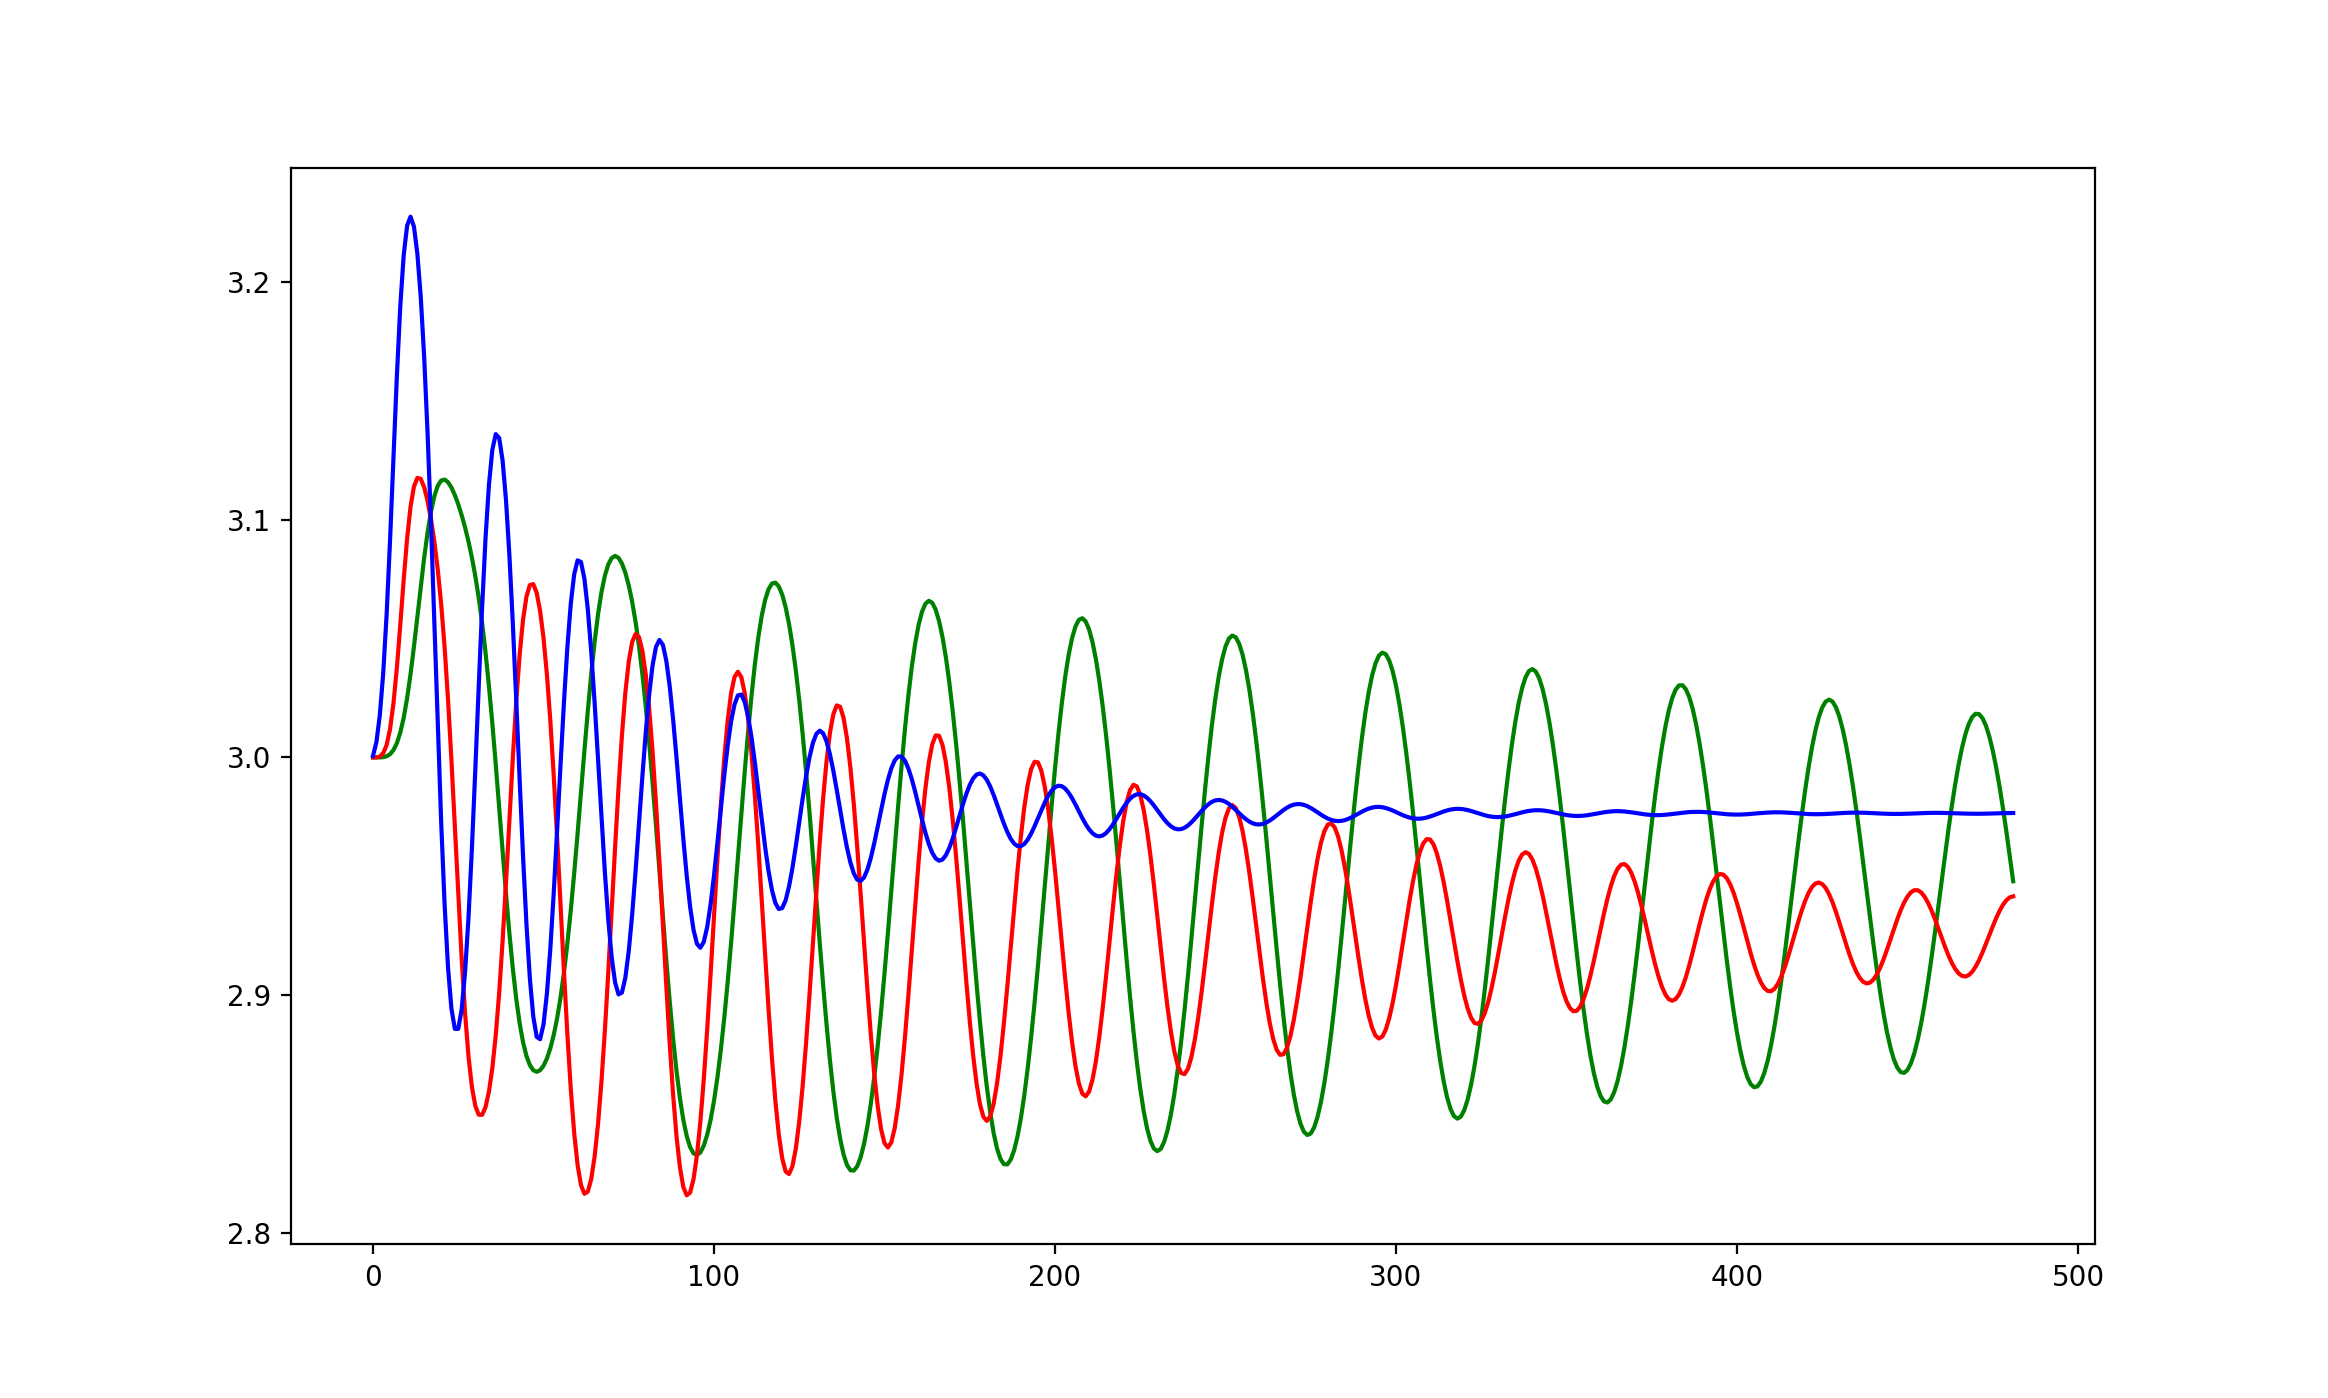
\includegraphics[width=0.5\textwidth]{../data/Figure_1}
 \caption{Shows the displacement in the $x$ direction (y axis) of the cart
 over time $t$ (x axis). Green is Euler's method, Red is the Modified Euler's method, and Blue is RK4.}
 \label{fig:yeet}
\end{figure}

Overall the results are quite nice. The standard Euler method works well and transfers
energy and momentum throughout the system as I would expect. However, it was difficult to
judge if results were correct, as the cart pole is a chaotic system. The changes in types
of numerical methods would make the chaotic nature of the system apparent after only a
few iterations, and that makes it hard to directly compare methods. Additionally,
the lack of a clear closed loop solution to the cart pole makes it difficult to compare
each individual result to a ground truth.

\begin{figure}[!ht]
 \centering
 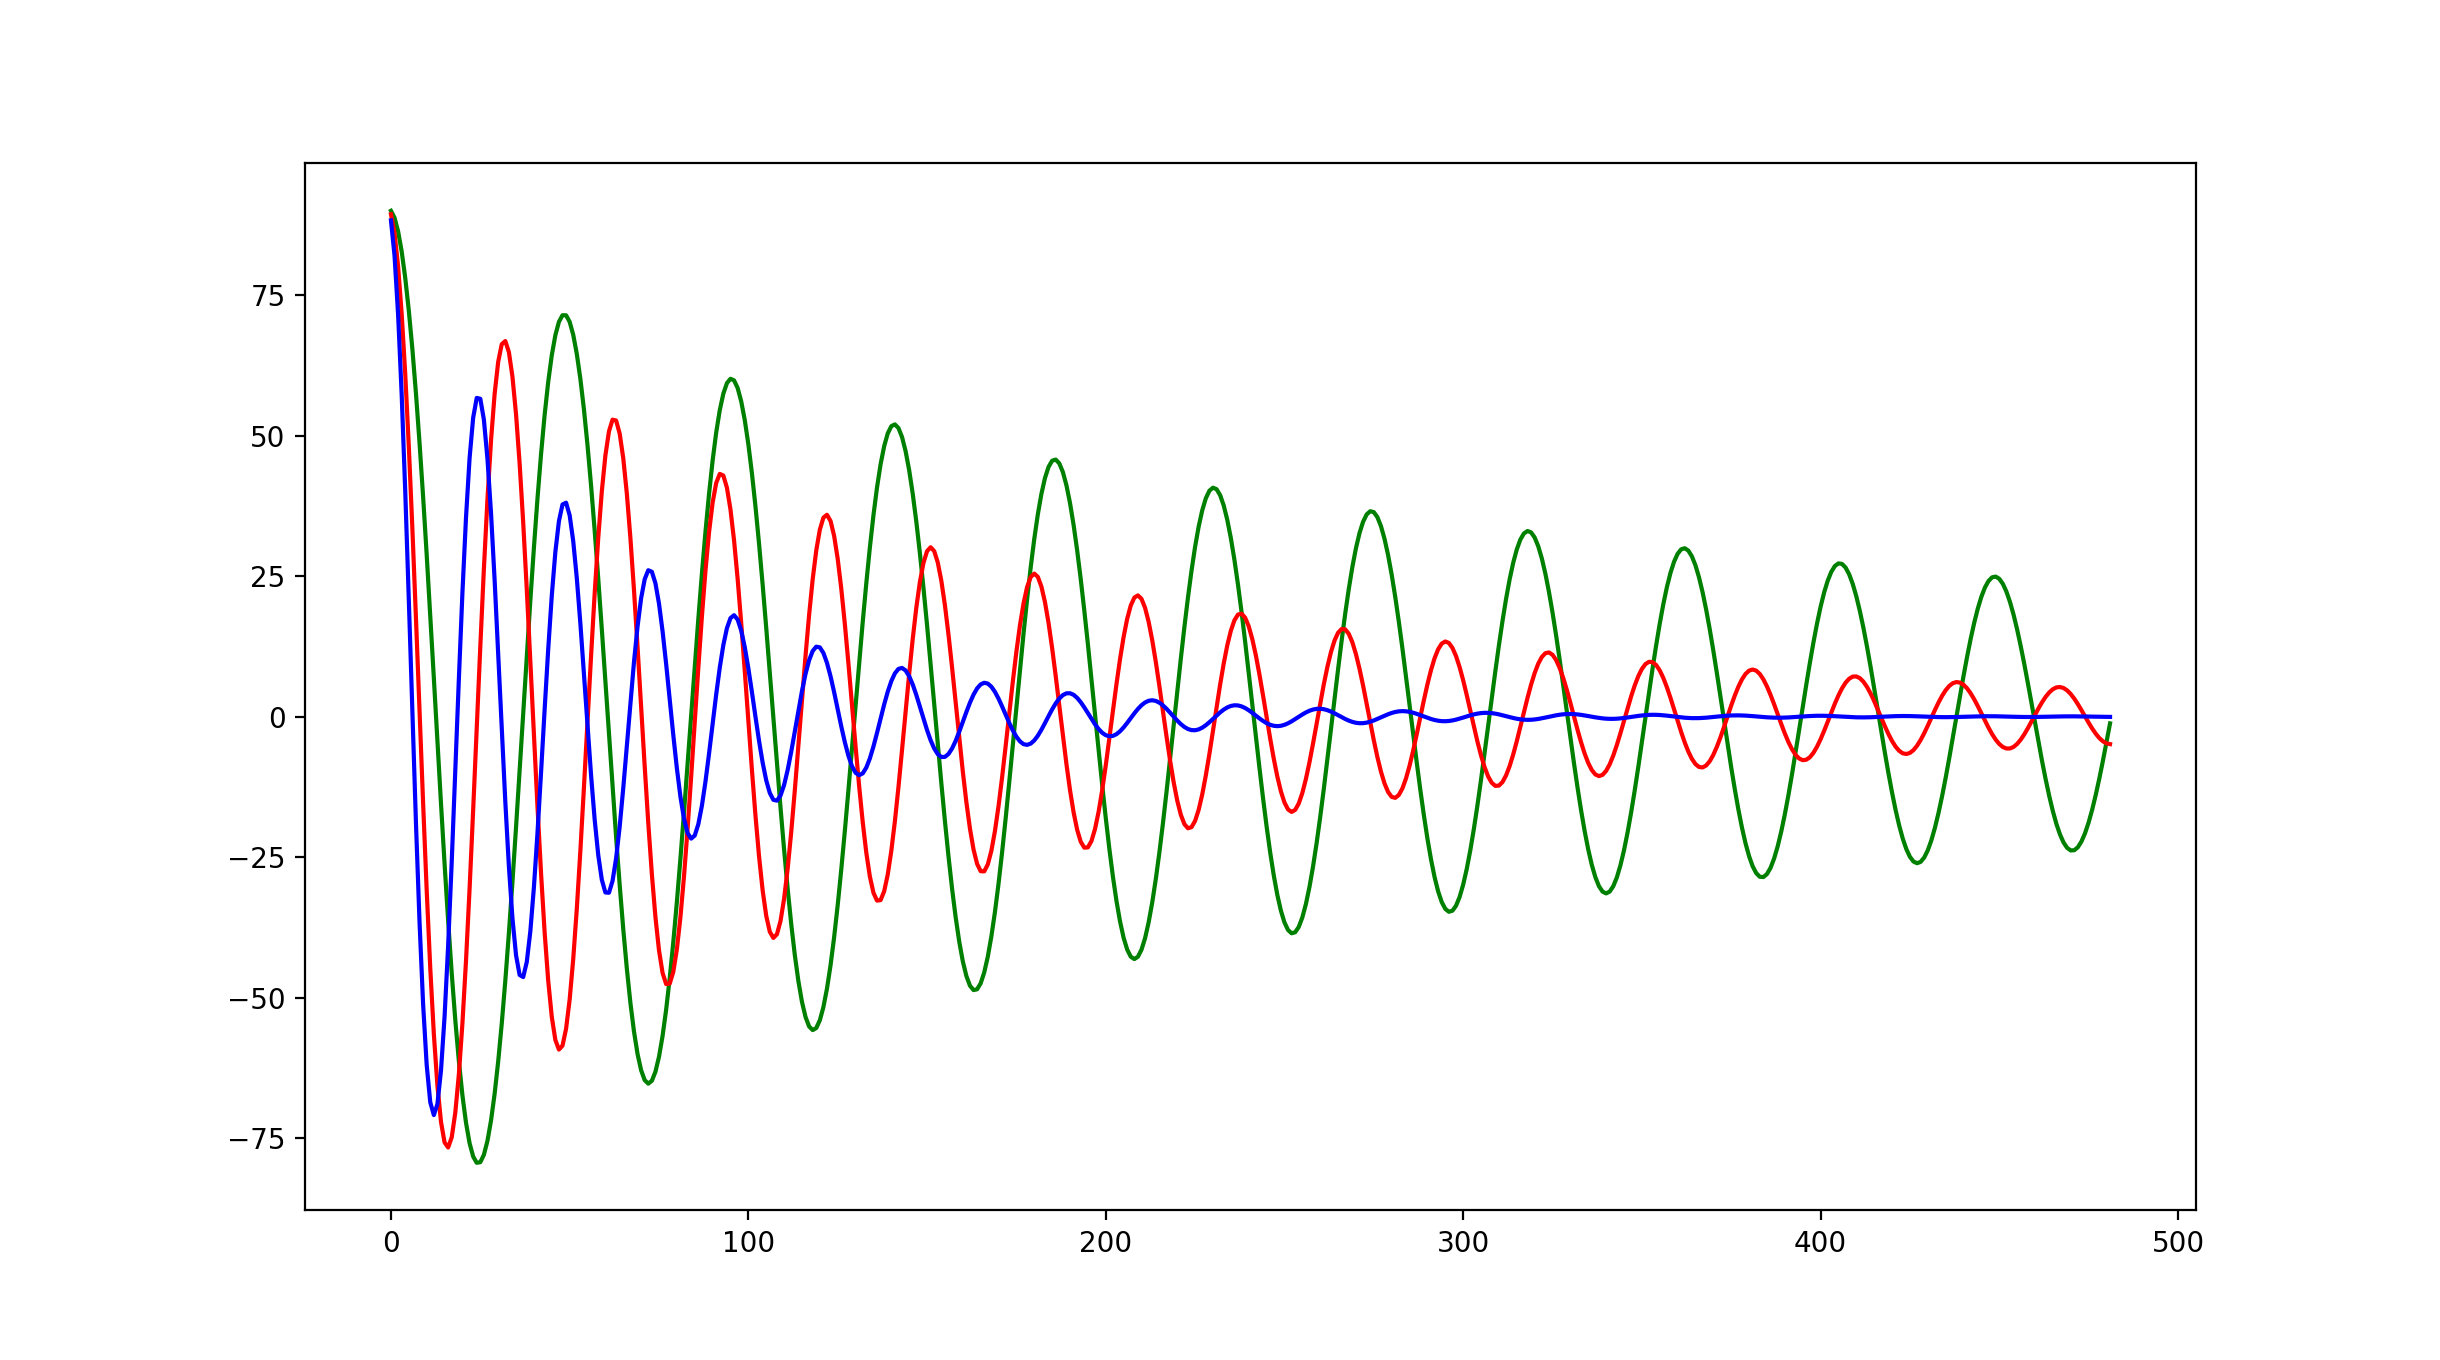
\includegraphics[width=0.5\textwidth]{../data/Figure_2}
 \caption{Shows the angle of the pole of the cart in radians (y axis) over
 time $t$ (x axis). Green is Euler's method, Red is the Modified Euler's method, and Blue is RK4.}
 \label{fig:yub}
\end{figure}

Many simulations, or models used for Trajectory Optimization, do not account for a dampening
factor or friction on the cart system. I attempted to model these, which is clear in Figures
4 and 5 as the amplitude clearly decreases over time. I do not think I adequately modeled
these dampening and friction forces, but as I mentioned above it is hard to tell due to the
chaotic nature of the Cart Pole. I would at least expect the rate of dampening to be similar
in each method, which is not something I see and leads me to believe there is some error associated
to that.

It is likely that I have not modeled the nuances of friction in the system correctly, and this could
be what is causing the divergent behavior with the amplitudes between methods. I assumed that I could model
both friction and the damping factor as a simple $- \mu \ddot{x}$ and $- \mu \ddot{\theta}$, where $mu$
is some constant coefficient. However, this is likely untrue, as friction is tied to the normal force. For
example, it is commonly know that $F_f \leq \mu F_n$ where $\mu$ is the coefficient of friction, $F_n$ is the
normal force, and $F_f$ is the true force of friction. This implies that the Cart Pole does not experience a
constant force due to friction (which is what I am currently modeling), as the normal force generated by
the pole will vary by its angle. This means
that there is a separate set of component forces that are not being modeled, as the swing-up of
the pole would cause the normal force $F_n$ to vary with the state of the pole. This could explain the strange
dampening of the modeled system and would need to be addressed to make the system more accurate. What could
complicate this further is that the cart pole cannot shake, as the motion of the cart is constrained
to the x axis. This is unrealistic in many ways. If the pole were to swing up fast enough and have a large
enough mass, it is realistic to expect the cart to shake an move within the plane of the pole - not
just the x axis.

\subsection{Future Work}

In the future I plan to derive the correct friction related equations as well as
attempt to control the cart pole system with the framework I have built. Once I can
formulate the system as an IVP, I will attempt to formulate it as a BVP. This is so
that I can perform Trajectory Optimization so that I can control the cart pole in
an upright state. The reason a BVP style solution is desired is because it can specify
a starting condition and an ending condition. It's possible that the Trajectory
Optimization could be combined with a simple controller.

\newpage

\bibliographystyle{IEEEtran}
\bibliography{sources}

\end{document}



























% yee
